\documentclass[12pt,a4paper]{ctexart}
\usepackage[margin=2.2cm]{geometry}
\usepackage{graphicx}
\usepackage{booktabs}
\usepackage{amsmath}
\usepackage{float}
\usepackage{hyperref}
\usepackage{xcolor}
\usepackage{listings}

\lstset{
  language=Verilog,
  basicstyle=\ttfamily\footnotesize,
  keywordstyle=\color{blue!70!black},
  commentstyle=\color{green!40!black},
  stringstyle=\color{orange!60!black},
  showstringspaces=false,
  breaklines=true,
  columns=fullflexible,
  keepspaces=true,
  frame=single,
  tabsize=4
}
\hypersetup{colorlinks=true,linkcolor=blue!50!black,urlcolor=blue!50!black}
\setlength{\emergencystretch}{2em}

\newcommand{\reporttitle}{计算机组成与系统结构专题实验\\实验二：时序逻辑设计}
\newcommand{\authname}{李祥熙}
\newcommand{\authid}{2234412799}
\newcommand{\class}{计算机2301}
\title{\reporttitle}
\author{姓名：\authname\quad 班级：\class\\学号：\authid}
\date{2026年11月11日}

\begin{document}
\maketitle
\tableofcontents
\newpage

\section{实验目的}
本实验使用Verilog描述时序逻辑电路，并在Vivado中通过行为仿真观察输入、时钟和输出之间的关系。主要目标如下：
\begin{itemize}
  \item 掌握SR锁存器和D锁存器的存储原理，区分电平敏感的锁存器与边沿触发的D触发器。
  \item 实现带使能、复位功能的存储单元，比较同步复位与异步复位，明确复位和使能的优先级。
  \item 实现并行寄存器、双向移位寄存器，以及以学号后两位99为模数的反馈清零计数器。
  \item 分别使用状态转移描述和触发器连接实现独热编码三分频电路，并实现检测二进制子序列01的Moore状态机。
  \item 编写自检查测试平台，结合波形和自动检查结果验证电路的功能与时序。
\end{itemize}

\section{实验过程}
\subsection{实验环境}
\begin{itemize}
  \item 操作系统：Microsoft Windows 11 Enterprise。
  \item 开发工具：AMD Vivado 2026.1，使用内置XSim仿真器。
  \item 硬件描述语言：Verilog；工程目标器件为\texttt{xc7a35tcsg324-1}。
  \item 仿真设置：时间单位为1 ns，时间精度为1 ps；周期性时钟的周期为10 ns，占空比为50\%。
  \item 验证方式：RTL行为仿真。本实验完成代码编译、展开和仿真，结果通过波形与测试平台共同检查。
\end{itemize}

\subsection{实现步骤}
首先完成D锁存器与D触发器的对比仿真，再补充SR锁存器和带复位、使能的存储单元。在此基础上，将单比特存储扩展到多位寄存器、移位寄存器和计数器，最后完成两个有限状态机任务。

设计文件与测试平台分别放在工程的设计源文件集和仿真源文件集中。每个测试平台单独作为仿真顶层，输入激励尽量安排在时钟下降沿或两个上升沿之间，输出检查安排在上升沿之后1 ns，避开非阻塞赋值尚未完成的时刻。检查采用\texttt{!==}比较，以便将意外的未知态和高阻态也识别出来。所有检查通过后打印\texttt{PASS}并结束仿真，发生不一致时调用\texttt{\$fatal}。

状态机采用组合逻辑计算下一状态，采用时钟触发的状态寄存器保存当前状态。组合过程使用阻塞赋值，时序过程使用非阻塞赋值，避免多个时钟过程之间因执行先后顺序产生竞争。

\section{实验内容}
\subsection{SR锁存器与D锁存器}
SR锁存器使用两个交叉反馈的或非门实现：
\begin{equation}
Q=\overline{R+Q_n},\qquad Q_n=\overline{S+Q}.
\end{equation}
其中，$Q_n$在正常存储状态下是$Q$的反相输出。其输入和状态关系如表\ref{tab:sr}所示。
\begin{table}[H]
\centering
\caption{或非门SR锁存器的功能}
\label{tab:sr}
\begin{tabular}{cccl}
\toprule
$S$ & $R$ & $(Q,Q_n)$ & 功能\\
\midrule
0 & 0 & 保持原值 & 存储\\
0 & 1 & $(0,1)$ & 复位\\
1 & 0 & $(1,0)$ & 置位\\
1 & 1 & $(0,0)$ & 禁止输入组合\\
\bottomrule
\end{tabular}
\end{table}
测试时先复位，再依次验证保持、置位、保持和禁止组合。离开禁止组合时先回到明确的复位输入，避免将同时撤销两个有效输入后的状态作为确定结果使用。

D锁存器使用使能信号控制数据通路。使能为1时，输出跟随输入；使能为0时，输出保持。带复位的版本将复位判断放在使能判断之前：
\begin{lstlisting}
always @(*) begin
    if (rst) q <= 1'b0;
    else if (en) q <= d;
end
\end{lstlisting}
这段代码没有最终的\texttt{else}分支，表示在复位和使能都无效时保留已有状态，因此会描述出锁存器。\texttt{rst}为高电平有效的异步复位，即使使能为0也能清零。

\subsection{D触发器、使能与复位}
D触发器仅在时钟上升沿采样输入。在没有复位的基本版本中，其核心描述为\texttt{always @(posedge clk)}。带控制端的版本提供\texttt{ASYNC\_RESET}参数，分别实例化同步复位和异步复位电路。

\begin{lstlisting}
// Asynchronous reset
always @(posedge clk or posedge rst)
    if (rst) q <= 1'b0;
    else if (en) q <= d;

// Synchronous reset
always @(posedge clk)
    if (rst) q <= 1'b0;
    else if (en) q <= d;
\end{lstlisting}
异步版本在复位上升沿立即清零；同步版本只有在时钟上升沿才检查复位。两个版本都采用“复位优先、使能其次”的顺序，因此\texttt{rst=1}与\texttt{en=1}同时成立时，清零优先于写入数据；\texttt{rst=0}且\texttt{en=0}时保持原值。

\subsection{并行寄存器与双向移位寄存器}
并行寄存器的位宽取8，各位共用同一时钟，在每个上升沿同时装入输入数据。寄存器使用内部变量\texttt{stored}保存内容，再通过输出控制信号\texttt{oe}决定是否驱动外部输出：
\begin{lstlisting}
always @(posedge clk) stored <= d;
assign q = oe ? {WIDTH{1'bz}} : stored;
\end{lstlisting}
\texttt{oe=1}时输出为高阻态，\texttt{oe=0}时输出内部存储值。存储和输出控制分开后，关闭输出不会清除数据，重新开放输出也无需等待下一次时钟。

双向移位寄存器的位宽取4，模式由两位信号\texttt{mode}选择。表\ref{tab:shift}给出了操作规则。本实现将复位端统一定义为高电平有效，与讲义中的移位寄存器Verilog示例一致。
\begin{table}[H]
\centering
\caption{4位双向移位寄存器的控制方式}
\label{tab:shift}
\begin{tabular}{ccl}
\toprule
复位 & \texttt{mode} & 操作\\
\midrule
1 & 任意 & 异步清零\\
0 & 00 & 保持原值\\
0 & 01 & 右移，$Q' = \{D_{sr},Q[3:1]\}$\\
0 & 10 & 左移，$Q' = \{Q[2:0],D_{sl}\}$\\
0 & 11 & 并行装入，$Q'=D$\\
\bottomrule
\end{tabular}
\end{table}
右移时串行输入\texttt{dsr}进入最高位，左移时\texttt{dsl}进入最低位。复位判断位于模式选择之前，因此清零不受当前模式和输入数据限制。

\subsection{模99反馈清零计数器}
学号为2234412799，后两位为99，因此计数器要求按$0,1,\ldots,98,0$循环。由于$2^6<99\leq2^7$，使用7位二进制存储单元。

底层二进制计数器采用类似74161的控制方式：\texttt{cr\_n}为低电平有效的异步清零，\texttt{pe\_n}为低电平有效的同步装入，\texttt{cep}和\texttt{cet}同时为1时允许计数。操作优先级为：异步清零、同步装入、使能计数、保持。

外层模块译码十进制99，并将译码结果反馈到低有效清零端：
\begin{lstlisting}
assign feedback_clear = (q == 7'd99);
assign internal_cr_n = cr_n && !feedback_clear;
assign tc = cet && (q == 7'd98);
\end{lstlisting}
计数到99时，反馈信号拉低内部清零端，计数值随即回到0，形成模99循环。正常稳定计数值共有99个。外层的\texttt{tc}用于指示末值98，底层二进制计数器自身的进位指示未作为外层输出使用。

零延时RTL仿真中，译码与清零在同一仿真时刻的不同delta周期内完成，反馈清零脉冲没有可见的纳秒级宽度。测试平台通过监听\texttt{feedback\_clear}的上升沿累加\texttt{wraps}，同时检查回绕后的稳定计数值，从而确认反馈动作确实发生。

\subsection{独热编码三分频状态机}
采用三个独热状态，按下式循环：
\begin{equation}
001\longrightarrow010\longrightarrow100\longrightarrow001,
\qquad Y=(S=001).
\end{equation}
复位进入001，输出为1。解除复位后，每个时钟上升沿前进一步，稳态下输出每三个时钟周期出现一次高电平，高电平持续一个时钟周期。

第一种实现使用\texttt{case}描述状态转移，\texttt{nextstate}由组合逻辑产生。第二种实现使用三个带异步置位、复位端的D触发器构成环形移位结构：
\begin{equation}
D_0=Q_2,\quad D_1=Q_0,\quad D_2=Q_1,\quad Y=Q_0.
\end{equation}
复位时将$Q_0$置1，将$Q_1$和$Q_2$清0，从而建立相同的初始状态。测试平台同时驱动两种实现，并逐周期比较三个状态位与输出。

\subsection{01子序列检测状态机}
序列检测器采用Moore结构，输出仅由当前状态决定。三个状态分别为：00表示尚未保留可匹配的0；01表示最近采样到0；10表示刚刚检测到01。状态转移如表\ref{tab:detect}所示，表中输出为当前状态对应的输出。
\begin{table}[H]
\centering
\caption{01检测器的状态转移}
\label{tab:detect}
\begin{tabular}{cccc}
\toprule
当前状态 & 输入$A$ & 下一状态 & 当前输出$Y$\\
\midrule
00 & 0 & 01 & 0\\
00 & 1 & 00 & 0\\
01 & 0 & 01 & 0\\
01 & 1 & 10 & 0\\
10 & 0 & 01 & 1\\
10 & 1 & 00 & 1\\
\bottomrule
\end{tabular}
\end{table}
在已采到0的状态下，下一次上升沿采到1便进入10，状态更新后输出1，并保持至下一个上升沿。检测状态遇到0又进入01，因此可以连续检测0101中的两次01。

除\texttt{case}实现外，还根据讲义给出的逻辑方程实现第二个版本：
\begin{equation}
S'_1=S_0A,\qquad S'_0=\overline A,\qquad Y=S_1.
\end{equation}
两个版本使用相同的复位和输入序列，测试平台将输出与“前一位为0且当前位为1”的参考结果比较，同时检查两个版本的状态是否一致。

\section{实验结果}
\subsection{锁存器与触发器的时序区别}
\begin{figure}[H]
\centering
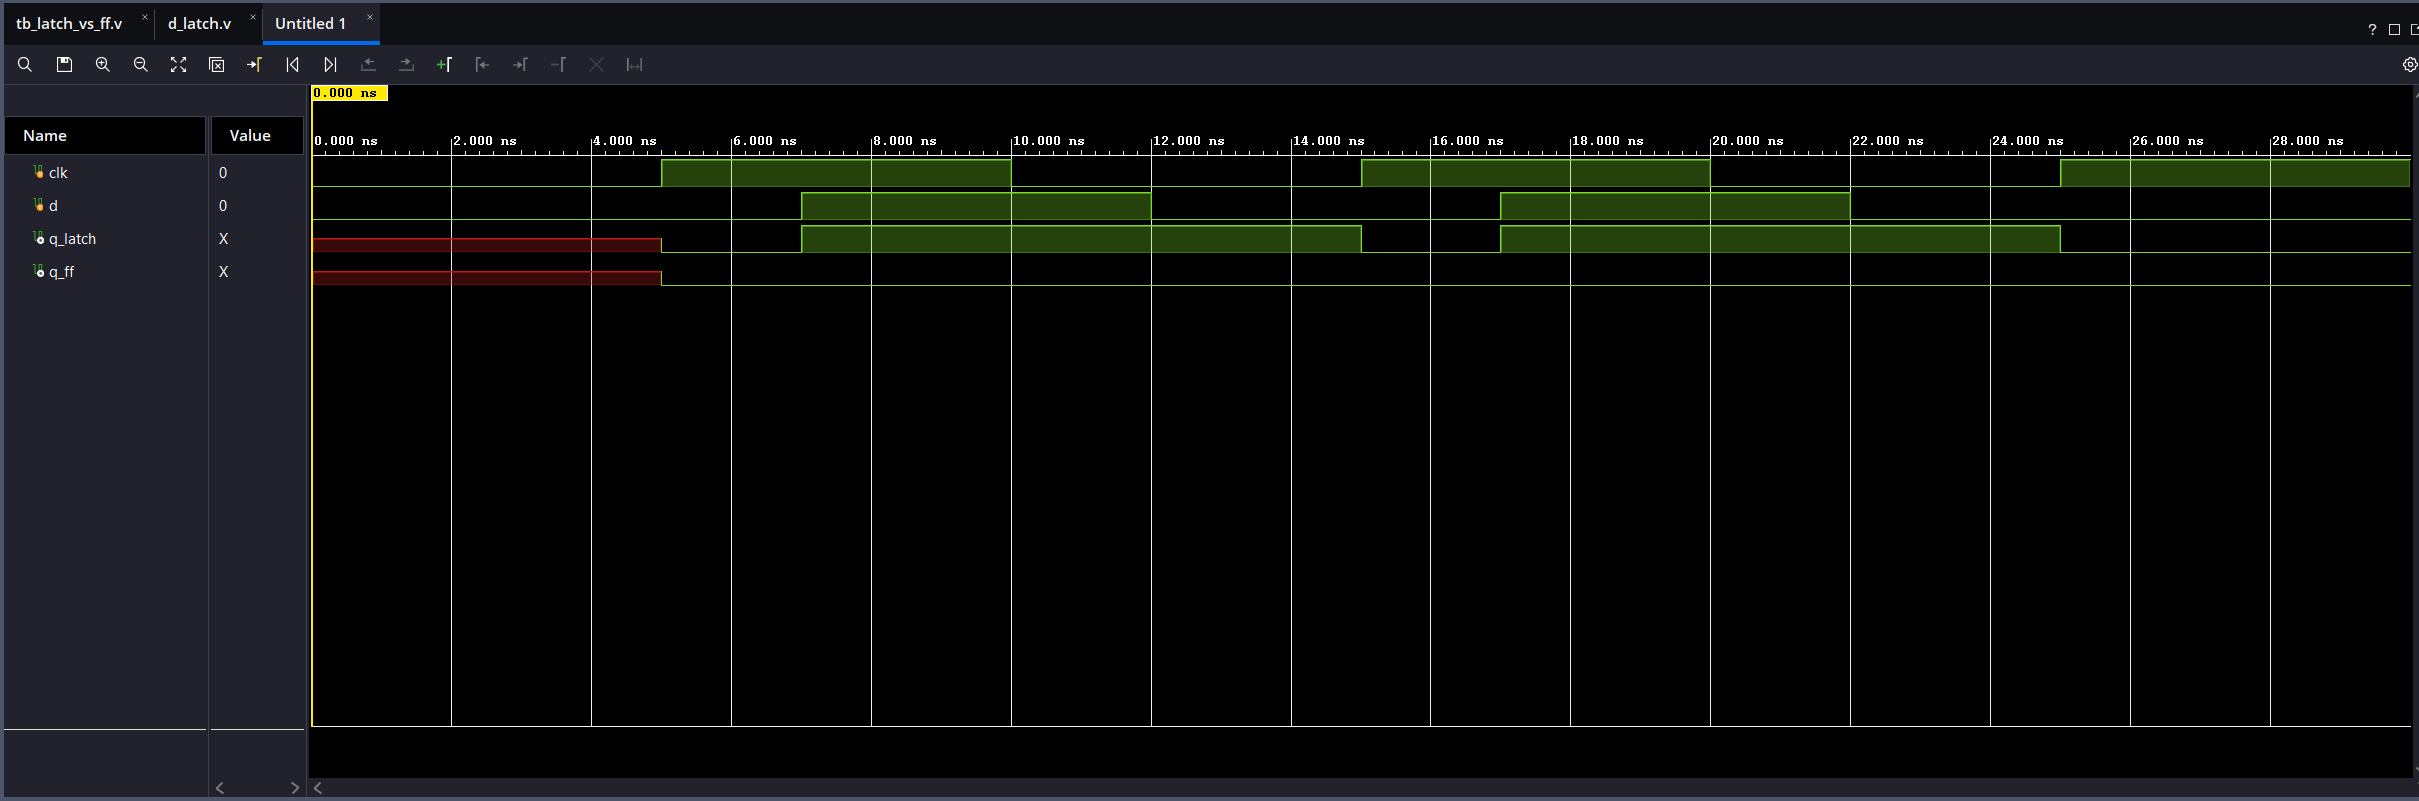
\includegraphics[width=\textwidth]{images/0-tb-latch-vs-ff.png}
\caption{D锁存器与D触发器对同一数据输入的响应}
\label{fig:latch-ff}
\end{figure}
图\ref{fig:latch-ff}中，两者在5 ns的时钟上升沿后都输出0。7 ns时，数据从0变为1，此时使能所接的时钟仍为高电平，锁存器立即输出1，而触发器继续保持0。12 ns时数据回到0，但时钟为低电平，锁存器保持先前的1；到15 ns上升沿，两者都取到0。17 ns和22 ns附近又出现同样的跟随与保持现象。仿真开始至首次有效采样前的未知态，来自基本模块没有设置初值或复位。

\begin{figure}[H]
\centering
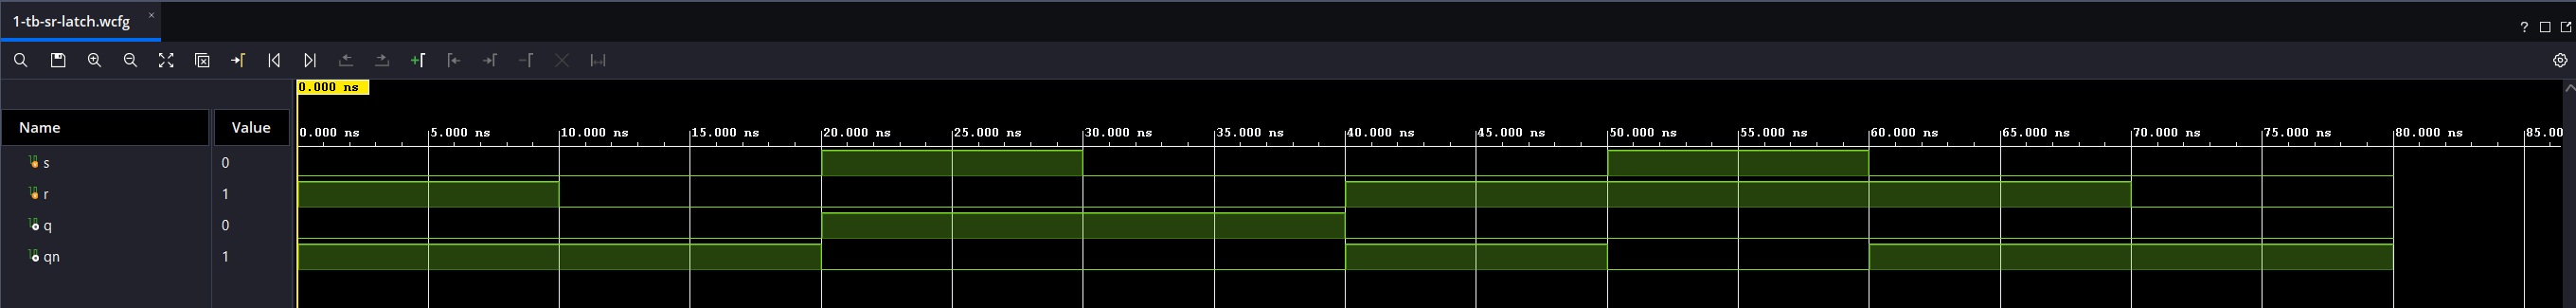
\includegraphics[width=\textwidth]{images/1-tb-sr-latch.png}
\caption{SR锁存器的复位、置位、保持与禁止组合}
\label{fig:sr}
\end{figure}
图\ref{fig:sr}中，0--10 ns通过$R=1$使$Q=0$，10--20 ns撤销复位后仍保持0；20--30 ns通过$S=1$将$Q$置1，30--40 ns在$S=R=0$时保持1。50--60 ns两个输入同时为1，两个输出同时变为0，符合或非门SR锁存器的禁止组合。随后先复位再保持，输出恢复到明确的$(0,1)$。测试平台共完成8组检查。

\begin{figure}[H]
\centering
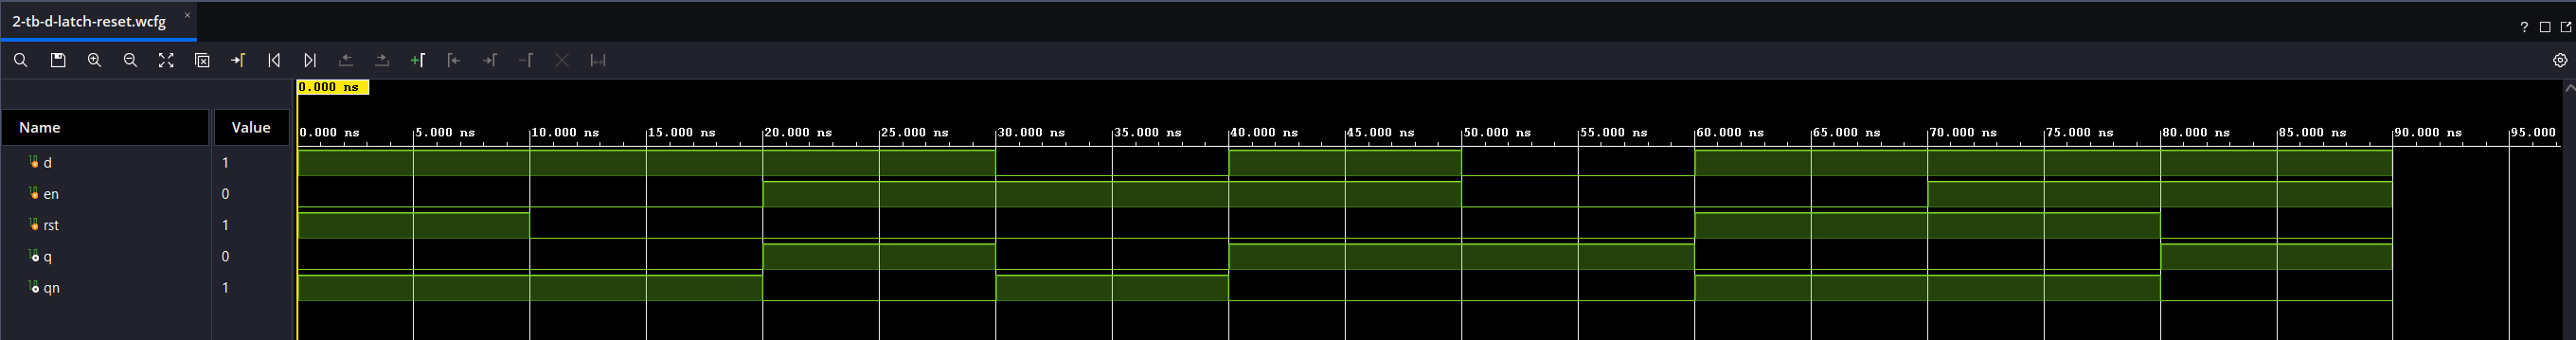
\includegraphics[width=\textwidth]{images/2-tb-d-latch-reset.png}
\caption{带异步复位的D锁存器}
\label{fig:latch-reset}
\end{figure}
图\ref{fig:latch-reset}中，20--50 ns使能为1，输出随数据依次取1、0、1。50 ns关闭使能后，虽然数据变0，输出仍保持1；60 ns置复位为1后立即清零。70--80 ns使能与复位同时有效，输出仍为0，说明复位优先。80 ns撤销复位且使能保持有效，输出重新跟随数据变为1。9组检查全部通过。

\subsection{使能、同步复位与异步复位}
\begin{figure}[H]
\centering
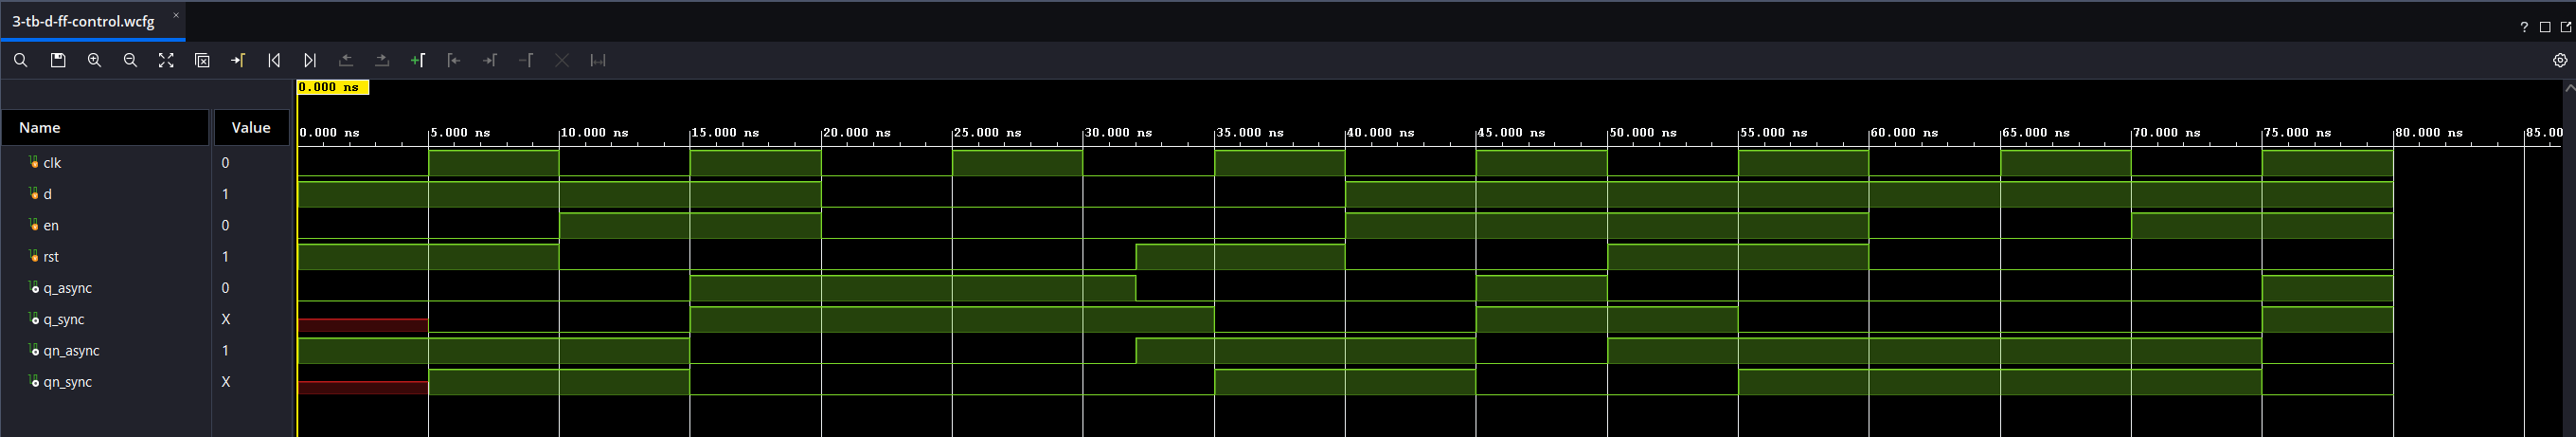
\includegraphics[width=\textwidth]{images/3-tb-d-ff-control.png}
\caption{同一激励下同步复位和异步复位触发器的比较}
\label{fig:ff-control}
\end{figure}
图\ref{fig:ff-control}中，15 ns两种触发器都装入1。20 ns后关闭使能并把输入改为0，25 ns上升沿输出仍为1，验证了使能无效时保持状态。32 ns在两个上升沿之间拉高复位，异步版本立即变0，同步版本继续保持1；35 ns上升沿到来后，同步版本才变0。此时使能仍为0，清零仍然执行，说明复位优先于使能。

之后重新使能并装入1，再令复位、使能和数据同时为1，两种输出均清零，进一步验证了控制优先级。\texttt{qn\_async}和\texttt{qn\_sync}分别与对应输出互补。9组使能、复位和时序检查均通过。

\subsection{并行寄存器与移位寄存器}
\begin{figure}[H]
\centering
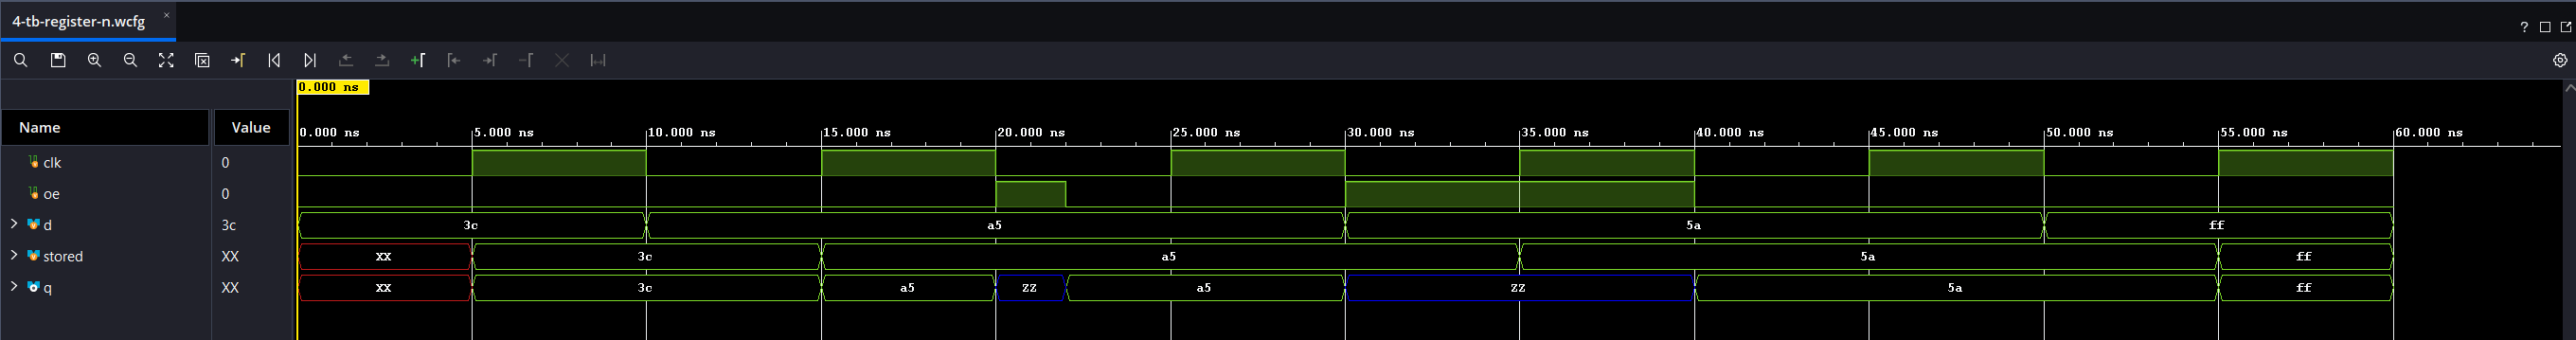
\includegraphics[width=\textwidth]{images/4-tb-register-n.png}
\caption{8位并行寄存器的数据存储和三态输出}
\label{fig:register}
\end{figure}
图\ref{fig:register}中的多位数据按十六进制显示。5 ns上升沿装入3C，10 ns输入改为A5时输出仍为3C，到15 ns才更新为A5。20 ns关闭输出后，\texttt{q}显示为ZZ，但内部\texttt{stored}仍为A5；22 ns重新开放输出，A5立即恢复。30--40 ns再次关闭输出，35 ns内部仍正常装入5A，40 ns开放输出时直接读出5A。最后55 ns装入FF。8组检查验证了并行装入、边沿间保持、高阻输出和恢复输出。

\begin{figure}[H]
\centering
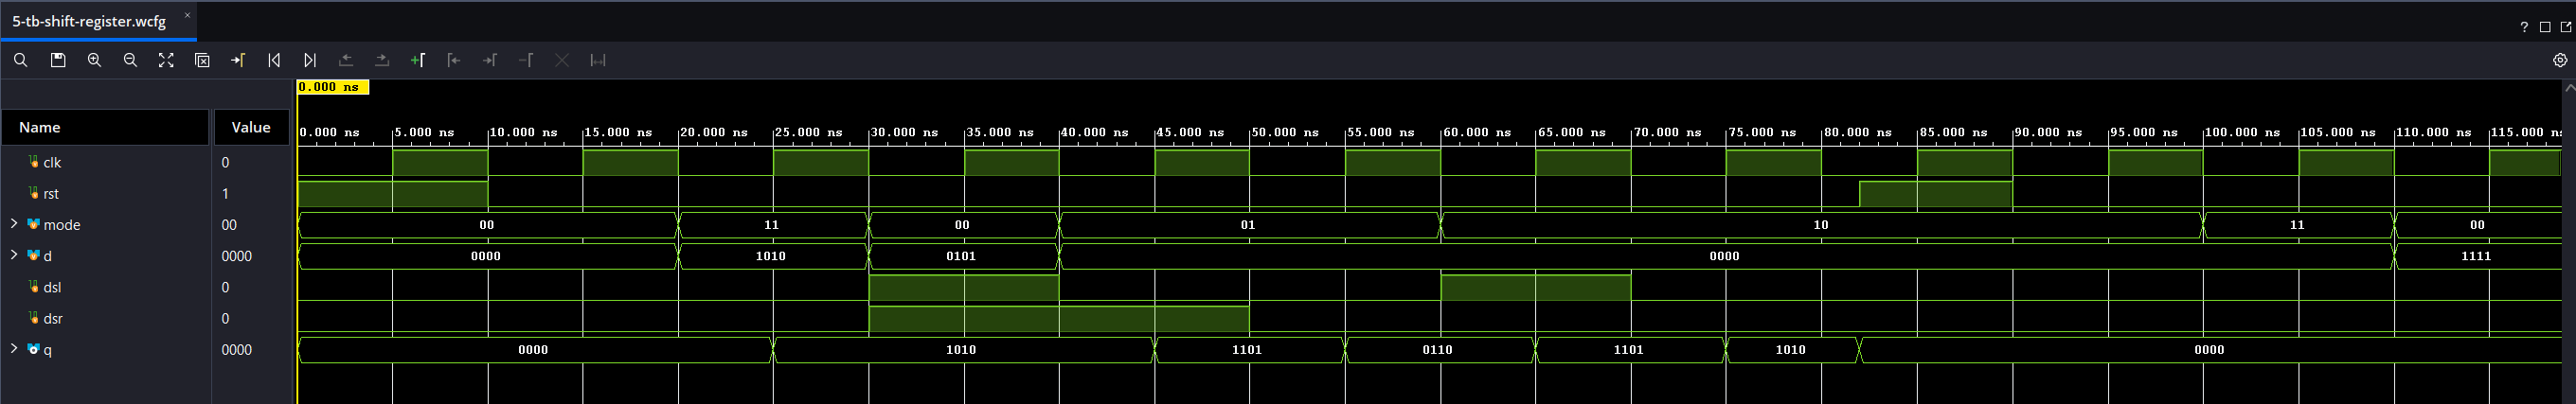
\includegraphics[width=\textwidth]{images/5-tb-shift-register.png}
\caption{4位双向移位寄存器的四种模式和异步清零}
\label{fig:shift}
\end{figure}
图\ref{fig:shift}中，25 ns并行装入1010；35 ns处于保持模式，输出不变。45 ns右移并从最高位移入1，得到1101；55 ns右移并移入0，得到0110。65 ns左移并从最低位移入1，得到1101；75 ns左移并移入0，得到1010。82 ns在非上升沿时刻拉高复位，输出立即清零。

上述定向激励之后，测试平台枚举16种初始字、4种模式和2种相关串行输入值，共128组模式与数据检查。每组先并行装入初始字，再执行指定模式，并将结果与移位、拼接运算得到的参考值比较，全部通过。

\subsection{模99计数、反馈清零与控制功能}
\begin{figure}[H]
\centering
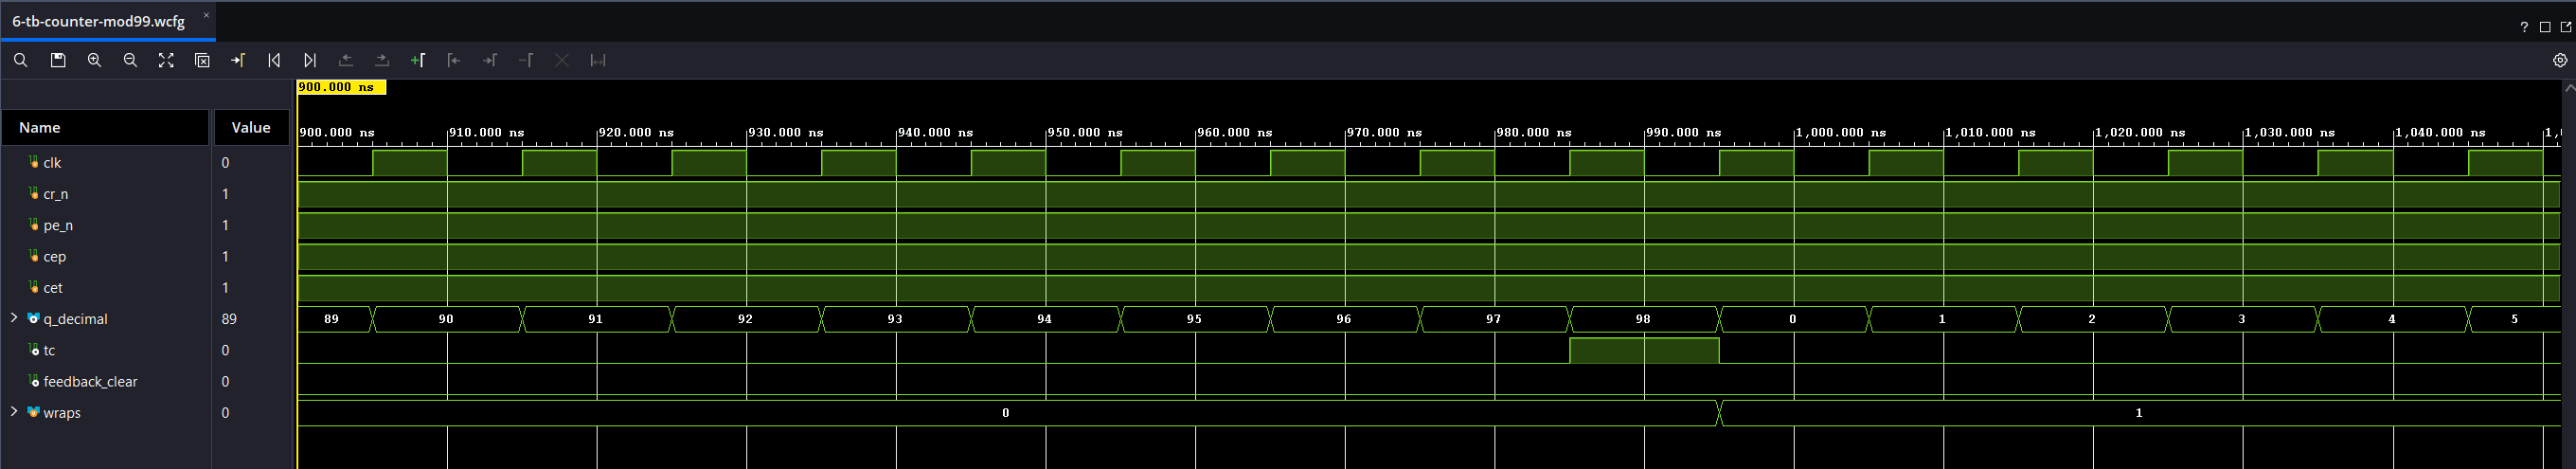
\includegraphics[width=\textwidth]{images/6-tb-counter-mod99.png}
\caption{模99计数器第一次自然回绕附近的波形}
\label{fig:counter-wrap}
\end{figure}
图\ref{fig:counter-wrap}中的计数值按十进制显示。计数值逐个增加，985 ns上升沿后达到98，此时末值指示\texttt{tc}有效。995 ns到来后，译码99触发反馈清零，稳定输出变为0，\texttt{wraps}从0增加到1；之后1005 ns继续计数为1。反馈脉冲在零延时波形中没有展开为持续的高电平，而事件计数与回绕结果共同反映了清零过程。

测试平台在保持使能有效的条件下连续检查198次计数，即两个完整模99周期，逐次将输出与$i\bmod99$比较，验证不是仅通过预装接近98的值来观察回绕。

\begin{figure}[H]
\centering
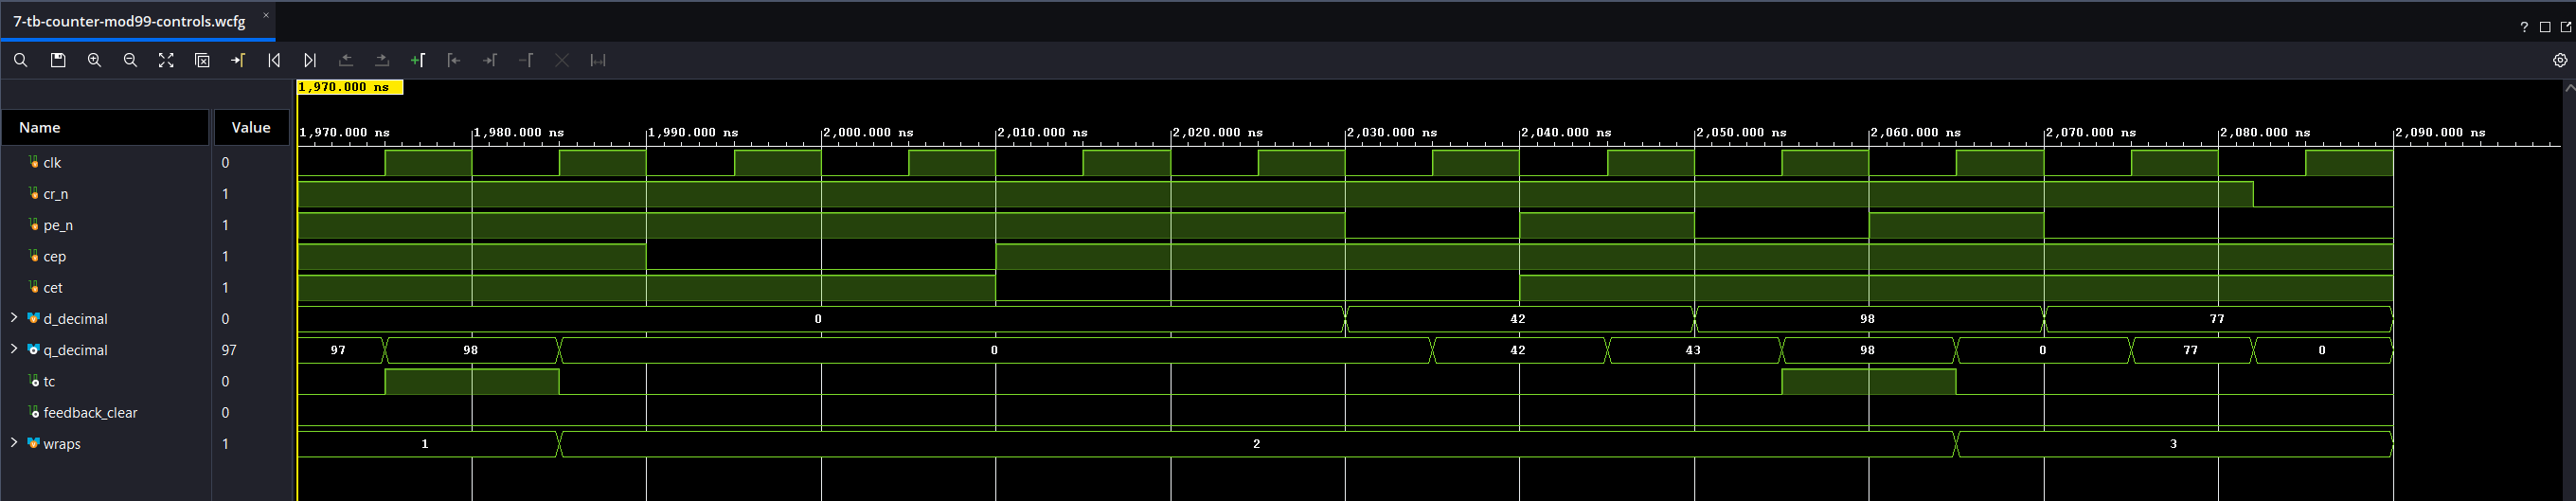
\includegraphics[width=\textwidth]{images/7-tb-counter-mod99-controls.png}
\caption{计数器的暂停、同步装入、末值回绕与异步清零}
\label{fig:counter-controls}
\end{figure}
图\ref{fig:counter-controls}中，1985 ns完成第二次自然回绕，\texttt{wraps}增加到2。随后分别将\texttt{cep}和\texttt{cet}置0，计数均保持不变。2035 ns在计数使能不完整时仍能装入42，说明同步装入优先于计数使能；2045 ns重新允许计数后得到43。

2055 ns预装98，2065 ns再次回绕到0，\texttt{wraps}增加到3。2075 ns装入77，2082 ns拉低外部清零端后立即变0，没有等待2085 ns上升沿。测试平台最终检查反馈事件总数恰为3，连续计数、使能、装入及复位检查全部通过。

\subsection{三分频状态机与触发器环形实现}
\begin{figure}[H]
\centering
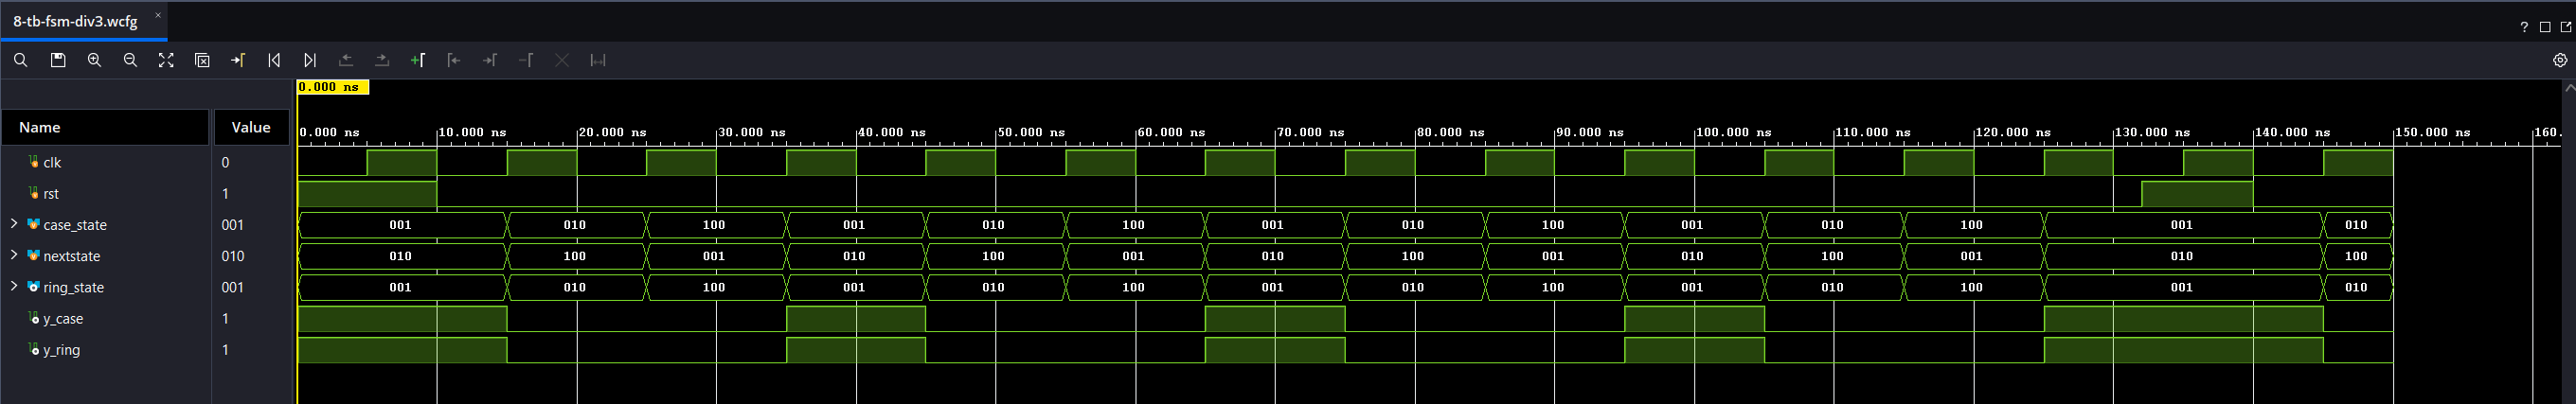
\includegraphics[width=\textwidth]{images/8-tb-fsm-div3.png}
\caption{独热编码三分频电路两种实现的状态和输出比较}
\label{fig:div3}
\end{figure}
图\ref{fig:div3}中，\texttt{case\_state}和\texttt{ring\_state}始终相同，按001、010、100循环。\texttt{nextstate}始终指向当前状态的后继状态，在时钟上升沿被状态寄存器采纳。\texttt{y\_case}与\texttt{y\_ring}也完全一致，在001状态输出1。

稳态高电平区间如35--45 ns、65--75 ns、95--105 ns，每次持续10 ns，相邻区间相隔30 ns，因此输出是每三个输入时钟出现一次、占空比为$1/3$的脉冲。132 ns再次拉高复位后，两个实现立即回到001，输出为1。测试平台完成12次连续状态转移比较，并检查了异步复位及复位后的转移，结果通过。

\subsection{01子序列检测结果}
\begin{figure}[H]
\centering
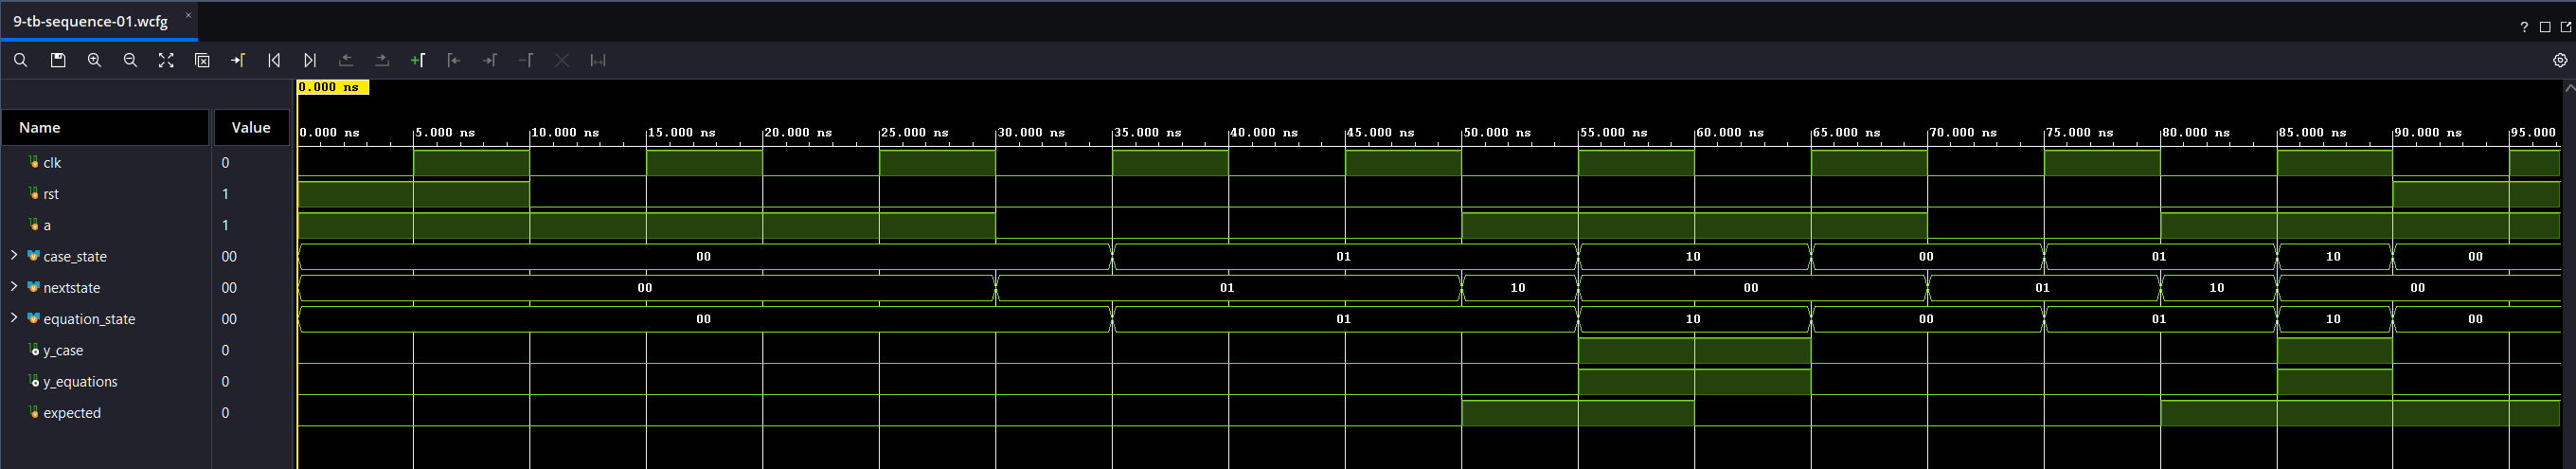
\includegraphics[width=\textwidth]{images/9-tb-sequence-01.png}
\caption{输入序列1001101的01子序列检测结果}
\label{fig:sequence}
\end{figure}
图\ref{fig:sequence}中，两个实现的状态和输出逐周期一致。复位后，测试序列在25--85 ns的七个上升沿依次采样，结果见表\ref{tab:sequence-result}。
\begin{table}[H]
\centering
\caption{示例序列的逐位采样与状态更新结果}
\label{tab:sequence-result}
\begin{tabular}{cccccccc}
\toprule
采样时刻/ns & 25 & 35 & 45 & 55 & 65 & 75 & 85\\
\midrule
输入$A$ & 1 & 0 & 0 & 1 & 1 & 0 & 1\\
更新后的状态 & 00 & 01 & 01 & 10 & 00 & 01 & 10\\
更新后的输出$Y$ & 0 & 0 & 0 & 1 & 0 & 0 & 1\\
\bottomrule
\end{tabular}
\end{table}
因此输入1001101对应输出0001001，两次01分别在第4位和第7位采样后被检测到。45 ns采到连续的第二个0时仍保持01，说明连续0不会丢失后续匹配机会；55 ns和85 ns进入10后输出为1。

示例之后，测试平台遍历全部64种六位二进制序列，每种序列前独立复位，共检查384个输入位。参考模型只记录前一位是否为0，与状态机的具体编码无关。每次采样后同时比较两个实现的输出、参考输出和内部状态，所有检查通过。

\subsection{自动检查汇总}
九个测试平台分别完成编译、展开和运行，实际输出的检查摘要如下：
\begin{lstlisting}[language={}]
Vivado XSim 2026.1 - Lab 2 self-checking behavioral simulations
Clock period: 10 ns. Student-ID modulus: 99.
PASS tb_counter_mod99: 198 natural counts, 3 feedback wraps, control checks
PASS tb_d_ff_control: 9 enable/reset/timing checks
PASS tb_d_latch_reset: 9 transparency/hold/reset checks
PASS tb_fsm_div3: case/ring equivalence, 12 transitions, asynchronous reset
PASS tb_latch_vs_ff: 7 latch/flip-flop timing checks
PASS tb_register_n: 8 capture/hold/high-impedance checks
PASS tb_sequence_01: sample 1001101 + all 64 six-bit streams (384 bits)
PASS tb_shift_register: directed timing + 128 mode/data/serial cases
PASS tb_sr_latch: 8 input/hold/forbidden checks
ALL 9 TESTBENCHES PASSED
\end{lstlisting}
其中，锁存器与触发器的检查重点是输入改变时刻和输出更新时刻的区别；寄存器检查存储与输出控制；计数器检查连续循环、反馈事件与控制优先级；状态机检查状态序列、输出和两种实现的一致性。汇总中的通过信息均在对应断言完成后打印，与前述波形结果一致。

\section{总结}
本实验完成了锁存器、触发器、寄存器、移位寄存器、模99反馈清零计数器和两类状态机任务，并通过九个自检查测试平台验证了功能与主要时序关系。

通过对比同一输入激励可以直接区分电平敏感与边沿采样：锁存器在使能有效的整个区间内透明，触发器只在有效时钟沿更新。使能决定时钟沿是否装入数据，而同步、异步复位的区别在于是否必须等待时钟沿。复位与使能同时存在时，通过先判断复位明确了清零优先级。

多位寄存器将单比特存储扩展为并行数据保存；移位寄存器通过模式选择实现保持、左右移位和装入。计数器在二进制累加基础上译码99并反馈清零，形成0至98的循环。有限状态机则将状态寄存器与组合转移逻辑分开，使三分频和序列检测的运行过程能够在内部状态波形中清楚观察。

验证过程中，测试输入安排在下降沿附近，输出在上升沿后检查，保证采样时序明确。序列检测测试还将复位后的空闲输入固定为1，避免正式测试序列前额外采入一个0。最终的连续计数检查、移位模式枚举和六位序列遍历均通过，说明所实现电路在给定激励下与参考行为一致。

\clearpage
\section*{附录：实验源代码与运行方法}
\addcontentsline{toc}{section}{附录：实验源代码与运行方法}
以下按设计模块和测试平台分组嵌入本次仿真实际使用的完整Verilog源代码。设计模块定义存储、控制和状态转移行为；测试平台产生激励并检查结果。复位极性、数据位宽和比较时刻均与正文说明一致。

\subsection*{A.1 设计模块}
\subsubsection*{A.1.1 \texttt{sr\_latch.v}}
\begin{lstlisting}
`timescale 1ns / 1ps
// Cross-coupled NOR latch. S=R=1 is forbidden (Q=QN=0).
module sr_latch(input wire s, r, output wire q, qn);
    nor (q, r, qn);
    nor (qn, s, q);
endmodule
\end{lstlisting}
两个或非门通过交叉反馈保存状态。这里直接保留两个独立输出，因此禁止组合时能够观察到两个输出同时为0。

\subsubsection*{A.1.2 \texttt{d\_latch.v}}
\begin{lstlisting}
`timescale 1ns / 1ps
//////////////////////////////////////////////////////////////////////////////////
// Company: 
// Engineer: 
// 
// Create Date: 11/11/2026 01:59:50 AM
// Design Name: 
// Module Name: d_latch
// Project Name: 
// Target Devices: 
// Tool Versions: 
// Description: 
// 
// Dependencies: 
// 
// Revision:
// Revision 0.01 - File Created
// Additional Comments:
// 
//////////////////////////////////////////////////////////////////////////////////


module d_latch (
    input  wire d,
    input  wire en,
    output reg  q
);
    always @(*) begin
        if (en)
            q <= d;
    end
endmodule
\end{lstlisting}
使能有效时装入数据，否则保留原值。该基本版本没有复位，用于与D触发器进行同输入时序比较。

\subsubsection*{A.1.3 \texttt{d\_ff.v}}
\begin{lstlisting}
`timescale 1ns / 1ps
//////////////////////////////////////////////////////////////////////////////////
// Company: 
// Engineer: 
// 
// Create Date: 11/11/2026 02:04:52 AM
// Design Name: 
// Module Name: d_ff
// Project Name: 
// Target Devices: 
// Tool Versions: 
// Description: 
// 
// Dependencies: 
// 
// Revision:
// Revision 0.01 - File Created
// Additional Comments:
// 
//////////////////////////////////////////////////////////////////////////////////


module d_ff (
    input  wire d,
    input  wire clk,
    output reg  q
);
    always @(posedge clk) begin
        q <= d;
    end
endmodule
\end{lstlisting}
只有时钟上升沿会更新输出，数据在其余时间改变不会立即传到输出。

\subsubsection*{A.1.4 \texttt{d\_latch\_reset.v}}
\begin{lstlisting}
`timescale 1ns / 1ps
module d_latch_reset(input wire d, en, rst, output reg q, output wire qn);
    always @(*) begin
        if (rst) q <= 1'b0;
        else if (en) q <= d;
        // No else: level-sensitive storage is intentional.
    end
    assign qn = ~q;
endmodule
\end{lstlisting}
复位判断位于使能之前，实现异步清零和复位优先；反相输出由当前存储值组合产生。

\subsubsection*{A.1.5 \texttt{d\_ff\_control.v}}
\begin{lstlisting}
`timescale 1ns / 1ps
// Reset has priority over enable. ASYNC_RESET=0 selects synchronous reset.
module d_ff_control #(parameter ASYNC_RESET = 1)(
    input wire clk, rst, en, d, output reg q, output wire qn
);
    generate
        if (ASYNC_RESET) begin : g_async
            always @(posedge clk or posedge rst)
                if (rst) q <= 1'b0;
                else if (en) q <= d;
        end else begin : g_sync
            always @(posedge clk)
                if (rst) q <= 1'b0;
                else if (en) q <= d;
        end
    endgenerate
    assign qn = ~q;
endmodule
\end{lstlisting}
参数选择生成同步或异步复位过程，两种实现均在复位无效且使能有效时装入数据。没有装入条件时保留状态。

\subsubsection*{A.1.6 \texttt{register\_n.v}}
\begin{lstlisting}
`timescale 1ns / 1ps
// OE=1 disables the external output, without erasing the stored data.
module register_n #(parameter WIDTH = 8)(
    input wire clk, oe,
    input wire [WIDTH-1:0] d,
    output wire [WIDTH-1:0] q
);
    reg [WIDTH-1:0] stored;
    always @(posedge clk) stored <= d;
    assign q = oe ? {WIDTH{1'bz}} : stored;
endmodule
\end{lstlisting}
内部存储在每个上升沿更新，输出使用独立的连续赋值实现高阻控制，因而关闭输出不会丢失数据。

\subsubsection*{A.1.7 \texttt{shift\_register.v}}
\begin{lstlisting}
`timescale 1ns / 1ps
// WIDTH >= 2. Active-high asynchronous clear, matching the slide's code.
module shift_register #(parameter WIDTH = 4)(
    input wire clk, rst,
    input wire [1:0] mode,
    input wire [WIDTH-1:0] d,
    input wire dsl, dsr,
    output reg [WIDTH-1:0] q
);
    always @(posedge clk or posedge rst) begin
        if (rst) q <= {WIDTH{1'b0}};
        else case (mode)
            2'b00: q <= q;
            2'b01: q <= {dsr, q[WIDTH-1:1]};
            2'b10: q <= {q[WIDTH-2:0], dsl};
            2'b11: q <= d;
        endcase
    end
endmodule
\end{lstlisting}
复位优先于四种模式。右移向最高位补入dsr，左移向最低位补入dsl，拼接顺序与正文的位序定义一致。

\subsubsection*{A.1.8 \texttt{counter\_mod99.v}}
\begin{lstlisting}
`timescale 1ns / 1ps
// 74161-style controls: active-low asynchronous clear and synchronous load.
module binary_counter #(parameter WIDTH = 7)(
    input wire clk, cr_n, pe_n, cep, cet,
    input wire [WIDTH-1:0] d,
    output reg [WIDTH-1:0] q,
    output wire tc
);
    always @(posedge clk or negedge cr_n) begin
        if (!cr_n) q <= {WIDTH{1'b0}};
        else if (!pe_n) q <= d;
        else if (cep && cet) q <= q + 1'b1;
    end
    assign tc = cet && (&q);
endmodule

// Required feedback-clear implementation: decode decimal 99, then clear.
// The decoded clear is a delta-cycle pulse in zero-delay RTL simulation.
module counter_mod99(
    input wire clk, cr_n, pe_n, cep, cet,
    input wire [6:0] d,
    output wire [6:0] q,
    output wire tc, feedback_clear
);
    wire internal_cr_n;
    wire unused_binary_tc;
    assign feedback_clear = (q == 7'd99);
    assign internal_cr_n = cr_n && !feedback_clear;
    binary_counter #(.WIDTH(7)) u_counter (
        .clk(clk), .cr_n(internal_cr_n), .pe_n(pe_n),
        .cep(cep), .cet(cet), .d(d), .q(q), .tc(unused_binary_tc)
    );
    // Terminal-count indication for modulo 99 (last stable count = 98).
    assign tc = cet && (q == 7'd98);
endmodule
\end{lstlisting}
第一个模块提供二进制计数、异步清零、同步装入和双使能控制。第二个模块将99译码反馈到清零端，并对稳定末值98产生指示。

\subsubsection*{A.1.9 \texttt{fsm\_div3.v}}
\begin{lstlisting}
`timescale 1ns / 1ps
module fsm_div3(input wire clk, rst, output wire y);
    reg [2:0] state, nextstate;
    always @(posedge clk or posedge rst)
        if (rst) state <= 3'b001;
        else state <= nextstate;
    always @(*) begin
        case (state)
            3'b001: nextstate = 3'b010;
            3'b010: nextstate = 3'b100;
            3'b100: nextstate = 3'b001;
            default: nextstate = 3'b001;
        endcase
    end
    assign y = (state == 3'b001);
endmodule

// Separate asynchronous preset/clear controls demonstrate slide 20.
// Clear has priority if both controls are asserted.
module d_ff_set_reset(input wire clk, aset, arst, d, output reg q);
    always @(posedge clk or posedge aset or posedge arst)
        if (arst) q <= 1'b0;
        else if (aset) q <= 1'b1;
        else q <= d;
endmodule

module ring_div3(input wire clk, rst, output wire y);
    wire [2:0] state;
    d_ff_set_reset u0(.clk(clk), .aset(rst), .arst(1'b0),
                      .d(state[2]), .q(state[0]));
    d_ff_set_reset u1(.clk(clk), .aset(1'b0), .arst(rst),
                      .d(state[0]), .q(state[1]));
    d_ff_set_reset u2(.clk(clk), .aset(1'b0), .arst(rst),
                      .d(state[1]), .q(state[2]));
    assign y = state[0];
endmodule
\end{lstlisting}
第一个模块使用组合下一状态逻辑与状态寄存器；后两个模块给出带置位、复位的触发器及三个触发器的环形连接。两种实现都复位到001。

\subsubsection*{A.1.10 \texttt{sequence\_01.v}}
\begin{lstlisting}
`timescale 1ns / 1ps
// Moore FSM: IDLE=00, SEEN_ZERO=01, FOUND=10. Output depends on state.
module sequence_01(input wire clk, rst, a, output wire y);
    localparam IDLE = 2'b00, SEEN_ZERO = 2'b01, FOUND = 2'b10;
    reg [1:0] state, nextstate;
    always @(posedge clk or posedge rst)
        if (rst) state <= IDLE;
        else state <= nextstate;
    always @(*) begin
        case (state)
            IDLE:      nextstate = a ? IDLE : SEEN_ZERO;
            SEEN_ZERO: nextstate = a ? FOUND : SEEN_ZERO;
            FOUND:     nextstate = a ? IDLE : SEEN_ZERO;
            default:   nextstate = IDLE;
        endcase
    end
    assign y = (state == FOUND);
endmodule

// Equivalent D-input equations from slide 22: S'={S0*A, ~A}, Y=S1.
module sequence_01_equations(input wire clk, rst, a, output wire y);
    reg [1:0] state;
    always @(posedge clk or posedge rst)
        if (rst) state <= 2'b00;
        else state <= {state[0] & a, ~a};
    assign y = state[1];
endmodule
\end{lstlisting}
第一个模块按三状态表转移，第二个模块按两个下一状态方程更新。两者输出都只取决于当前状态。

\subsection*{A.2 自检查测试平台}
\subsubsection*{A.2.1 \texttt{tb\_sr\_latch.v}}
\begin{lstlisting}
`timescale 1ns / 1ps
module tb_sr_latch;
    reg s, r;
    wire q, qn;
    sr_latch dut(.s(s), .r(r), .q(q), .qn(qn));
    task check;
        input es, er, eq, eqn;
        begin
            s = es; r = er; #10;
            if ({q, qn} !== {eq, eqn})
                $fatal(1, "SR mismatch S=%b R=%b Q=%b QN=%b", s,r,q,qn);
        end
    endtask
    initial begin
        check(0,1,0,1); // initialize by resetting
        check(0,0,0,1); // hold zero
        check(1,0,1,0); // set
        check(0,0,1,0); // hold one
        check(0,1,0,1); // reset
        check(1,1,0,0); // forbidden NOR-latch condition
        check(0,1,0,1); // leave forbidden condition through a defined reset
        check(0,0,0,1);
        $display("PASS tb_sr_latch: 8 input/hold/forbidden checks");
        $finish;
    end
endmodule
\end{lstlisting}
测试依次覆盖复位、保持、置位和禁止组合，再通过明确复位退出禁止组合。每组激励等待10 ns后比较两个输出。

\subsubsection*{A.2.2 \texttt{tb\_latch\_vs\_ff.v}}
\begin{lstlisting}
`timescale 1ns / 1ps
//////////////////////////////////////////////////////////////////////////////////
// Company: 
// Engineer: 
// 
// Create Date: 11/11/2026 02:06:31 AM
// Design Name: 
// Module Name: tb_latch_vs_ff
// Project Name: 
// Target Devices: 
// Tool Versions: 
// Description: 
// 
// Dependencies: 
// 
// Revision:
// Revision 0.01 - File Created
// Additional Comments:
// 
//////////////////////////////////////////////////////////////////////////////////


module tb_latch_vs_ff;
    reg clk;
    reg d;

    wire q_latch;
    wire q_ff;

    d_latch u_latch (
        .d(d), .en(clk), .q(q_latch)
    );

    d_ff u_ff (
        .d(d), .clk(clk), .q(q_ff)
    );

    initial clk = 0;
    always #5 clk = ~clk;  // 10 ns period

    initial begin
        #6;
        if ({q_latch,q_ff} !== 2'b00) $fatal(1,"Initial capture failed");
        #2;
        if ({q_latch,q_ff} !== 2'b10) $fatal(1,"Transparency check failed");
        #5;
        if ({q_latch,q_ff} !== 2'b10) $fatal(1,"Hold check failed");
        #3;
        if ({q_latch,q_ff} !== 2'b00) $fatal(1,"Edge capture failed");
        #2;
        if ({q_latch,q_ff} !== 2'b10) $fatal(1,"Second transparency failed");
        #5;
        if ({q_latch,q_ff} !== 2'b10) $fatal(1,"Second hold failed");
        #3;
        if ({q_latch,q_ff} !== 2'b00) $fatal(1,"Final capture failed");
        $display("PASS tb_latch_vs_ff: 7 latch/flip-flop timing checks");
    end

    initial begin
        d = 0;
        #7  d = 1;
        #5  d = 0;
        #5  d = 1;
        #5  d = 0;
        #8;

        $finish;
    end
endmodule
\end{lstlisting}
同一个时钟同时驱动锁存器使能和触发器时钟，数据在非边沿时刻改变。独立检查过程在7个观测点比较输出，原有波形激励保持不变。

\subsubsection*{A.2.3 \texttt{tb\_d\_latch\_reset.v}}
\begin{lstlisting}
`timescale 1ns / 1ps
module tb_d_latch_reset;
    reg d, en, rst;
    wire q, qn;
    d_latch_reset dut(.d(d),.en(en),.rst(rst),.q(q),.qn(qn));
    task check;
        input ed, een, erst, expected;
        begin
            d=ed; en=een; rst=erst; #10;
            if ({q,qn} !== {expected,~expected})
                $fatal(1,"Latch mismatch d=%b en=%b rst=%b q=%b",d,en,rst,q);
        end
    endtask
    initial begin
        check(1,0,1,0);
        check(1,0,0,0);
        check(1,1,0,1);
        check(0,1,0,0);
        check(1,1,0,1);
        check(0,0,0,1);
        check(1,0,1,0); // reset overrides hold
        check(1,1,1,0); // reset overrides data and enable
        check(1,1,0,1);
        $display("PASS tb_d_latch_reset: 9 transparency/hold/reset checks");
        $finish;
    end
endmodule
\end{lstlisting}
9组输入逐项检查透明、保持和异步复位，包含使能有效与复位同时有效的情况。

\subsubsection*{A.2.4 \texttt{tb\_d\_ff\_control.v}}
\begin{lstlisting}
`timescale 1ns / 1ps
module tb_d_ff_control;
    reg clk=0;
    reg rst, en, d;
    wire q_async, q_sync, qn_async, qn_sync;
    d_ff_control #(.ASYNC_RESET(1)) u_async(
        .clk(clk),.rst(rst),.en(en),.d(d),.q(q_async),.qn(qn_async));
    d_ff_control #(.ASYNC_RESET(0)) u_sync(
        .clk(clk),.rst(rst),.en(en),.d(d),.q(q_sync),.qn(qn_sync));
    always #5 clk=~clk;
    task check;
        input ea, es;
        begin
            if ({q_async,q_sync,qn_async,qn_sync} !== {ea,es,~ea,~es})
                $fatal(1,"FF mismatch t=%0t async=%b sync=%b",$time,q_async,q_sync);
        end
    endtask
    initial begin
        rst=1; en=0; d=1;
        @(posedge clk); #1; check(0,0);
        @(negedge clk); rst=0; en=1;
        @(posedge clk); #1; check(1,1);
        @(negedge clk); en=0; d=0;
        @(posedge clk); #1; check(1,1); // disabled: hold
        @(negedge clk); #2; rst=1;
        #1; check(0,1); // at 33 ns, between rising edges
        @(posedge clk); #1; check(0,0); // at 36 ns, sync catches up
        @(negedge clk); rst=0; en=1; d=1;
        @(posedge clk); #1; check(1,1);
        @(negedge clk); rst=1; en=1; d=1;
        @(posedge clk); #1; check(0,0); // reset priority
        @(negedge clk); rst=0; en=0;
        @(posedge clk); #1; check(0,0);
        @(negedge clk); en=1;
        @(posedge clk); #1; check(1,1);
        #4;
        $display("PASS tb_d_ff_control: 9 enable/reset/timing checks");
        $finish;
    end
endmodule
\end{lstlisting}
两个参数实例共享输入，检查使能保持、32 ns异步清零、35 ns同步清零和复位优先级，同时检查反相输出。

\subsubsection*{A.2.5 \texttt{tb\_register\_n.v}}
\begin{lstlisting}
`timescale 1ns / 1ps
module tb_register_n;
    reg clk=0;
    reg oe;
    reg [7:0] d;
    wire [7:0] q;
    register_n dut(.clk(clk),.oe(oe),.d(d),.q(q));
    always #5 clk=~clk;
    task check;
        input [7:0] expected;
        begin
            if(q !== expected) $fatal(1,"Register q=%h expected=%h",q,expected);
        end
    endtask
    initial begin
        oe=0; d=8'h3c;
        @(posedge clk); #1; check(8'h3c);
        @(negedge clk); d=8'ha5; #1; check(8'h3c);
        @(posedge clk); #1; check(8'ha5);
        @(negedge clk); oe=1; #1; check(8'hzz);
        #1; oe=0; #1; check(8'ha5); // output restored before next clock
        @(negedge clk); oe=1; d=8'h5a;
        @(posedge clk); #1; check(8'hzz); // storage still captures data
        @(negedge clk); oe=0; #1; check(8'h5a);
        @(negedge clk); d=8'hff;
        @(posedge clk); #1; check(8'hff);
        #4;
        $display("PASS tb_register_n: 8 capture/hold/high-impedance checks");
        $finish;
    end
endmodule
\end{lstlisting}
测试数据在边沿之间保持不变的输出，以及输出关闭期间仍能写入内部存储的行为。高阻态使用四态比较检查。

\subsubsection*{A.2.6 \texttt{tb\_shift\_register.v}}
\begin{lstlisting}
`timescale 1ns / 1ps
module tb_shift_register;
    reg clk=0;
    reg rst, dsl, dsr;
    reg [1:0] mode;
    reg [3:0] d;
    wire [3:0] q;
    integer m, value, serial_bit;
    reg [3:0] expected;
    shift_register dut(.clk(clk),.rst(rst),.mode(mode),.d(d),
                       .dsl(dsl),.dsr(dsr),.q(q));
    always #5 clk=~clk;
    task check;
        input [3:0] e;
        begin if(q !== e) $fatal(1,"Shift mode=%b q=%b expected=%b",mode,q,e); end
    endtask
    task step;
        input [1:0] op;
        input [3:0] data;
        input sl, sr;
        input [3:0] result;
        begin
            @(negedge clk); mode=op; d=data; dsl=sl; dsr=sr;
            @(posedge clk); #1; check(result);
        end
    endtask
    initial begin
        rst=1; mode=0; d=0; dsl=0; dsr=0;
        #1; check(0);
        @(negedge clk); rst=0;
        step(3,4'b1010,0,0,4'b1010);
        step(0,4'b0101,1,1,4'b1010);
        step(1,0,0,1,4'b1101);
        step(1,0,0,0,4'b0110);
        step(2,0,1,0,4'b1101);
        step(2,0,0,0,4'b1010);
        @(negedge clk); #2; rst=1; #1; check(0);
        @(negedge clk); rst=0;
        // Check every starting word, mode, and relevant serial-input value.
        for(value=0;value<16;value=value+1)
            for(m=0;m<4;m=m+1)
                for(serial_bit=0;serial_bit<2;serial_bit=serial_bit+1) begin
                    step(3,value,0,0,value);
                    case(m)
                        0: expected=value;
                        1: expected=(value>>1) | (serial_bit<<3);
                        2: expected=(value<<1) | serial_bit;
                        3: expected=15-value;
                    endcase
                    step(m,15-value,serial_bit,serial_bit,expected);
                end
        $display("PASS tb_shift_register: directed timing + 128 mode/data/serial cases");
        $finish;
    end
endmodule
\end{lstlisting}
先执行正文波形中的定向操作，再枚举16种初始字、4种模式和2种相关串行输入值，逐项计算期望结果。

\subsubsection*{A.2.7 \texttt{tb\_counter\_mod99.v}}
\begin{lstlisting}
`timescale 1ns / 1ps
module tb_counter_mod99;
    reg clk=0;
    reg cr_n, pe_n, cep, cet;
    reg [6:0] d;
    wire [6:0] q;
    wire tc, feedback_clear;
    integer i, expected, wraps=0;
    counter_mod99 dut(.clk(clk),.cr_n(cr_n),.pe_n(pe_n),.cep(cep),.cet(cet),
                      .d(d),.q(q),.tc(tc),.feedback_clear(feedback_clear));
    always #5 clk=~clk;
    always @(posedge feedback_clear) wraps=wraps+1;
    task check;
        input [6:0] e;
        begin
            if(q !== e || tc !== (cet && (e==98)))
                $fatal(1,"Counter q=%d expected=%d tc=%b",q,e,tc);
        end
    endtask
    initial begin
        cr_n=0; pe_n=1; cep=1; cet=1; d=0;
        #1; check(0);
        @(negedge clk); cr_n=1;
        // Two complete natural cycles, without loading near the boundary.
        for(i=1;i<=198;i=i+1) begin
            @(posedge clk); #1; expected=i%99; check(expected);
        end
        @(negedge clk); cep=0;
        repeat(2) begin @(posedge clk); #1; check(0); end
        @(negedge clk); cep=1; cet=0;
        repeat(2) begin @(posedge clk); #1; check(0); end
        @(negedge clk); pe_n=0; d=42; // load overrides disabled counting
        @(posedge clk); #1; check(42);
        @(negedge clk); pe_n=1; cet=1;
        @(posedge clk); #1; check(43);
        @(negedge clk); pe_n=0; d=98;
        @(posedge clk); #1; check(98);
        @(negedge clk); pe_n=1;
        @(posedge clk); #1; check(0);
        @(negedge clk); pe_n=0; d=77;
        @(posedge clk); #1; check(77);
        @(negedge clk); #2; cr_n=0; #1; check(0);
        if(wraps !== 3) $fatal(1,"Expected 3 feedback-clear events, got %0d",wraps);
        #7;
        $display("PASS tb_counter_mod99: 198 natural counts, 3 feedback wraps, control checks");
        $finish;
    end
endmodule
\end{lstlisting}
先检查198次连续计数，再检查两个使能端、低有效装入和异步清零。监听反馈事件的计数最终应为3，输出值在delta周期结束后比较。

\subsubsection*{A.2.8 \texttt{tb\_fsm\_div3.v}}
\begin{lstlisting}
`timescale 1ns / 1ps
module tb_fsm_div3;
    reg clk=0;
    reg rst;
    wire y_case, y_ring;
    integer i;
    reg [2:0] expected;
    fsm_div3 u_case(.clk(clk),.rst(rst),.y(y_case));
    ring_div3 u_ring(.clk(clk),.rst(rst),.y(y_ring));
    always #5 clk=~clk;
    task check;
        input [2:0] e;
        begin
            if(u_case.state !== e || u_ring.state !== e ||
               y_case !== (e==3'b001) || y_ring !== (e==3'b001))
                $fatal(1,"Divider state=%b ring=%b expected=%b",u_case.state,u_ring.state,e);
        end
    endtask
    initial begin
        rst=1; #1; check(3'b001);
        @(negedge clk); rst=0;
        expected=3'b001;
        for(i=0;i<12;i=i+1) begin
            expected={expected[1:0],expected[2]};
            @(posedge clk); #1; check(expected);
        end
        @(negedge clk); #2; rst=1; #1; check(3'b001);
        @(negedge clk); rst=0;
        @(posedge clk); #1; check(3'b010);
        #4;
        $display("PASS tb_fsm_div3: case/ring equivalence, 12 transitions, asynchronous reset");
        $finish;
    end
endmodule
\end{lstlisting}
同时实例化case状态机和三个触发器组成的环形电路，连续比较12次状态转移，并在非时钟沿检查异步复位。

\subsubsection*{A.2.9 \texttt{tb\_sequence\_01.v}}
\begin{lstlisting}
`timescale 1ns / 1ps
module tb_sequence_01;
    reg clk=0;
    reg rst, a;
    wire y_case, y_equations;
    reg previous_zero, expected;
    reg [6:0] sample;
    integer i, pattern, bit_index;
    sequence_01 u_case(.clk(clk),.rst(rst),.a(a),.y(y_case));
    sequence_01_equations u_equations(.clk(clk),.rst(rst),.a(a),.y(y_equations));
    always #5 clk=~clk;
    task send_bit;
        input value;
        begin
            @(negedge clk); a=value;
            expected=previous_zero && value;
            @(posedge clk); #1;
            if(y_case !== expected || y_equations !== expected ||
               u_case.state !== u_equations.state)
                $fatal(1,"Detector a=%b y=%b equation=%b expected=%b",a,y_case,y_equations,expected);
            previous_zero=~value;
        end
    endtask
    task reset_dut;
        begin
            @(negedge clk); rst=1; a=1; previous_zero=0;
            #1;
            if(y_case !== 0 || y_equations !== 0) $fatal(1,"Detector reset failed");
            @(negedge clk); rst=0;
        end
    endtask
    initial begin
        rst=1; a=1; previous_zero=0; expected=0; sample=7'b1001101;
        @(negedge clk); rst=0;
        // Handout example first, for a readable screenshot: Y=0001001.
        for(i=6;i>=0;i=i-1) send_bit(sample[i]);
        // All 64 six-bit streams, including repeated/overlapping 0101 cases.
        for(pattern=0;pattern<64;pattern=pattern+1) begin
            reset_dut;
            for(bit_index=5;bit_index>=0;bit_index=bit_index-1)
                send_bit((pattern>>bit_index)&1);
        end
        #4;
        $display("PASS tb_sequence_01: sample 1001101 + all 64 six-bit streams (384 bits)");
        $finish;
    end
endmodule
\end{lstlisting}
先输入讲义示例1001101，再遍历全部六位序列。参考模型只记录前一位是否为0，并在采样后比较两个实现的状态与输出。复位后的空闲输入为1。

\end{document}
